\documentclass[conference]{IEEEtran}
\usepackage{graphicx,amsmath,amssymb,booktabs,xcolor,etoolbox}
\newcommand{\need}[1]{\textcolor{red}{[NEED NUMBER: #1]}}
\newcommand{\num}[1]{\textcolor{orange}{[\detokenize{#1}]}}
\newcommand{\chk}[1]{\textcolor{blue}{[CHECK: #1]}}
\newcommand{\prereg}[1]{\textcolor{violet}{[PREREG: #1]}}
\newcommand{\IfFig}[2]{\IfFileExists{#1}{\includegraphics[width=\linewidth]{#1}}{\fbox{\parbox{0.9\linewidth}{\centering #2}}}}
\newif\ifsupp\suppfalse % supplement is a separate target: tectonic supp.tex (supp.tex defines \buildsupp and inputs this file)
\ifdefined\buildsupp\supptrue\fi
\ifsupp
\makeatletter
\newlabel{tab:t1}{{I}{1}}\newlabel{tab:t2}{{II}{1}}\newlabel{fig:f2}{{2}{1}}
\newlabel{sec:discussion}{{V}{1}}\newlabel{sec:method}{{III}{1}}\newlabel{sec:deviations}{{III-F}{1}}
\makeatother
\renewcommand{\thesection}{S-\Roman{section}}
\renewcommand{\thetable}{S\arabic{table}}
\renewcommand{\thefigure}{S\arabic{figure}}
\title{Supplementary Material for Impossible or Just Unexpected? Testing What the Surprise of a Public V-JEPA Checkpoint Detects}
\else
\title{Impossible or Just Unexpected? Testing What the Surprise of a Public V-JEPA Checkpoint Detects}
\fi
\author{\IEEEauthorblockN{Anand Rodriguez Menon}\IEEEauthorblockA{Department of Computer Science and Engineering\\Amrita Vishwa Vidyapeetham, Amritapuri, India\\am.sc.u4cse25025@am.students.amrita.edu}}
\begin{document}
\ifsupp
\maketitle
\section{Deviations, amendments and known design weaknesses}
\label{sec:supp-dev}
Each item below departs from the plan or limits what a result can show, and is carried into the Discussion of the main text. Section~III-F of the main text summarises them; nothing here changes a number reported there.

\emph{Checkpoint and accuracy gap (G1$'$).} The original gate required V-JEPA pairwise accuracy of at least 90\% on IntPhys dev. It was not met: the public ViT-L checkpoint reaches 81.7\% (ViT-H 88.3\%, tie-half under the pre-registered threshold; strict 87.8\%). The checkpoints behind the published results are not released, and the cause of the gap is unexplained; we do not claim to have reproduced the published accuracy (98\%, ViT-H, context length tuned per property). Scoring the released per-video surprise files with our own code gives 96.7\% for ViT-H and 89.4\% for ViT-L (our recomputation, \texttt{verify/released\_dev\_accuracy.md}; not figures from Garrido et al.). The replacement gate G1$'$ checks the pipeline only (preprocessing against the official configuration, an independent surprise recomputation on three videos, bitwise-identical inputs); all three passed. No released per-video surprise values exist for the public checkpoints. An earlier fixed threshold of $10^{-4}$ gave slightly different tie-half figures for some baselines; it was superseded and is not quoted.

\emph{Positive controls (G2 not met).} Vertical flip raised M1's surprise in 21.1\% of possible videos (CI 14.7 to 28.1) against the 80\% gate; horizontal flip 38.6\%, time reversal 60.8\%, and pairwise accuracy on vertically flipped pairs is 83.9\%, not lower than clean. We did not tune or rerun the edits. By human decision (Q10-A, 2026-10-08) the study continued with G2 not met. Three readings remain open: the edits may not be strong violations for this model; the pipeline may be insensitive; or the signal may act as a splice-discontinuity detector, since impossible dev videos are frame splices of possible ones, which flips and reversals do not produce. The last fits the comparison with the copy-last-frame baseline B2 (76.1\%, against M1's 80.8\% in fp16; paired difference +4.7 pp, interval $-$1.1 to 10.6 pp, including zero). M1's sensitivity to physical impossibility, as opposed to splice discontinuities, is therefore not established here. A random-weight network (M0r) responds to vertical flip in 87.8\% of videos where about 50\% was expected; the pre-registered claim that M0r detection is near 0.5 by construction was wrong for max aggregation, and the M1 minus M0r contrast is not a measure of learned sensitivity.

\emph{Magnitude matching in H2.} The frozen event rule looks for the first frame where the whole-frame pixel divergence $D(t)$ exceeds $2/255$. We expected it never to fall back; it fell back to a seeded random onset in 178 of 180 pairs. This is a failure of the rule (a local object change moves a whole-frame mean very little), not a finding that no event exists. Matching is therefore over a random window, abrupt edits are placed at that time, and the median matched magnitude is 0.33 of 255 grey levels, so the edits are near-threshold and nearly invisible. The rule was run as written, with human approval. At mid strength the achieved-to-target ratio met the target for local lighting, jolt and zoom and missed it for global lighting, where the required gain is below the 8-bit rounding step: in 84 of 180 entries the edit is a no-op, so $A$ is reported with and without that type. Both baselines fall below 0.5 (B1 0.335, B2 0.379): matching on mean absolute difference does not equalise what pixel detectors see; we did not verify why.

\emph{M2 wrapper.} The first V-JEPA~2 run queried the predictor with mask token index~1, but only token~0 is trained in the released checkpoint. After the freeze, we changed the index to~0 (one token, human-approved, logged before any edited M2 output was opened) and reran the clean split: 46.9\% before, 60.8\% after. Both are reported. At 60.8\% M2 is below the 80\% threshold, so it is not H1-eligible and its edited runs are descriptive.

\emph{Invariance for M1 is descriptive.} The dither floor, the verdict flip rate under an invisible $\pm1$ grey-level dither, must stay below 10\% for a confirmatory reading. For M1 it is 21.5\% (tie-half) and 15.6\% (strict); part of the tie-half figure is pairs entering or leaving the tie band, so the strict figure is less inflated. It was measured in fp16 only; a same-input fp16 versus fp32 comparison changes 2.8\% of verdicts, so precision alone does not produce it. Every edit is therefore read through its accuracy change and its flip rate relative to the floor, and we do not assign the analysis driver's verdict labels. For JPEG, the cluster and sign tests disagree in the strict convention (0.0088 versus 0.1151; tie-half $<$0.0001 and 0.018), so its verdict depends on the convention. For zoom, a retention rule excludes pairs where the crop keeps less than 90\% of the violation support, leaving 112 of 180; the driver reads a derived subset of the retention file, with no code change.

\emph{Frame-rate edit (design error).} The pre-registered edit halves the frame rate of a clip already sampled at every second frame, which reproduces the skip-4 clean reference exactly (bit-identical outputs). Its zero change cannot be read as invariance. It is an error in our pre-registration, not a finding, and is excluded from all counts of invariant edits.

\emph{Other.} The dose-response (A3) uses Holm over 30 tests for H1 edits (the pre-registration names 21, but only 15 graded cells exist) and over 24 for the H2 cells (12 cells, two contrasts); no cell changes significance under the conservative 42-slot variant for H1. M1's H1 eligibility was judged on the fp32 clean run (81.7\%); all contrasts use fp16 (clean 80.8\%). The G1$'$ ladder compares ViT-L in fp32 with ViT-H in fp16. Kernel bundles were rebuilt from clean trees at later commits and the commit allowlist extended, with differences limited to files the pre-registration exempts plus the M2 model file; the per-pair matching file was generated after the freeze from dev pixels only; the Colab fallback was not used, so all runs share one GPU type and precision.

\emph{Exploratory analyses} are labelled wherever they appear: an onset-aligned specificity variant using the splice time derived from dev pixels, a hold-based frame-rate edit that differs from the skip-4 reference, and a paired check of M0r's shift under vertical flip. The IntPhys~2 Main clean run is descriptive, as pre-registered.

\section{Exploratory analyses}
\label{sec:supp-expl}
These were run after the confirmatory results were seen and are exploratory (Table~\ref{tab:t7}).

\emph{Onset-aligned specificity.} Using the splice time derived from prefix-sharing frames of the dev pixels (no fallbacks), the AUROC of M1 is 0.392 (0.354 to 0.428), 0.392 without global lighting, with $A_0$ unchanged at 0.722. It is lower than with the random windows (0.546). The baselines are still below 0.5 (0.327 and 0.381), $D_1=$+0.065 (0.023 to 0.109) and $D_2=$+0.011 ($-$0.026 to 0.051; Holm $p=$0.277). The detection precondition is unchanged ($A_0$ as above), so the outcome of the rule does not change. That the baselines remain below 0.5 is consistent with mean-pixel matching not equalising what pixel detectors see; we did not verify this.

\emph{Corrected frame-rate edit.} A hold-based halving that differs from the skip-4 reference changes accuracy by +1.9 pp ($-$3.3 to 7.5) with a flip rate of 20.0\%, against a floor of 21.5\%; this is within the floor.

\IfFileExists{tables/t7_exploratory.tex}{\begin{table}[t]
\caption{EXPLORATORY (post-hoc, not pre-registered). (a) H2 re-run with the event onset defined from the data (first frame at which the impossible and possible videos differ), instead of the frozen threshold that found an onset in only 2 of 180 pairs; 60 of the 180 events are transient. $A$ = specificity AUROC [95\% CI]; $D_1$, $D_2$ vs B1, B2 (Holm-2 $p$). (b) Halve-and-hold edit for H1 (frame rate halved, clip length held), replacing the frame-rate-halving edit, which was a design error.}
\label{tab:t7}
\centering\scriptsize
\setlength{\tabcolsep}{2.6pt}
\begin{tabular}{@{}lc@{}}
\toprule
\multicolumn{2}{@{}l}{\textbf{EXPLORATORY (a) onset-aligned H2, M1}} \\
\midrule
$A$ [95\% CI] & 0.392 [0.354, 0.428] \\
$A_0$ (clean, same aggregation) [CI] & 0.722 [0.653, 0.789] \\
$A$ without lighting\_global [CI] & 0.392 [0.357, 0.426] \\
$D_1$ vs B1 [CI] (Holm $p$) & 0.065 [0.023, 0.109] (0.003) \\
$D_2$ vs B2 [CI] (Holm $p$) & 0.011 [$-$0.026, 0.051] (0.28) \\
$A_{B1}$, $A_{B2}$ & 0.327, 0.381 \\
$A$ by type (lg / ll / jolt / zoom) & 0.390 / 0.460 / 0.400 / 0.317 \\
\midrule
\multicolumn{2}{@{}l}{\textbf{EXPLORATORY (b) halve-and-hold, M1}} \\
\midrule
$\Delta$Acc [CI] (pp) & +1.9 [$-$3.3, 7.5] \\
Flip rate (\%) / floor $f_0$ (\%) & 20.0 / 21.5 \\
Flip $-$ $f_0$ [CI] (pp) & $-$1.5 [$-$8.2, 5.2] \\
\bottomrule
\end{tabular}
\end{table}
}{\par\noindent\textbf{[TODO table T7: tables/t7\_exploratory.tex missing]}\par}

\emph{Random-weight network under vertical flip.} A paired check on the stored arrays shows that M0r's surprise shifts systematically in one direction under vertical flip, opposite to M1's shift for the same videos, and that the shift is not a tie or noise effect. Its cause is not established.

\emph{M2 dose-response (descriptive).} All M2 dose cells are seed~1 only. JPEG and zoom were not run at low or mid strength. The scope gap is the unrun group \texttt{m2\_dose\_inv\_s1\_b} (JPEG and zoom, low and mid) and the seed-2 and seed-3 groups, none of which were run because of the GPU quota. M2 is H1-ineligible, so the M2 dose-response is descriptive throughout and no dose cell supports a confirmatory claim. For the pooled H2 dose, M2's $A$ is 0.483 (0.434 to 0.533), 0.449 (0.403 to 0.497) and 0.420 (0.375 to 0.468) at low, mid and high strength, with $A_0=$0.600 throughout, so $A$ stays below 0.5 and falls with strength. Against the pixel baselines, $D_1$ is 0.117, 0.125 and 0.145, and $D_2$ is 0.054 ($-$0.001 to 0.108), 0.074 and 0.103; the detection precondition is unmet at every strength, so these contrasts are not read as specificity. On the H1 side, blur raises M2's accuracy by +15.8, +18.6 and +12.8 pp at low, mid and high strength with flip rates of 35.6\%, 34.4\% and 42.2\% against its 24.6\% floor, while noise at mid strength lowers it by 8.1 pp ($-$13.9 to $-$2.2) with a flip rate of 30.0\%. The Holm families are 22 tests for H1 and 24 (cell level) or 6 (pooled) for H2.

\section{Additional tables and figures}
\label{sec:supp-add}
\IfFileExists{tables/t3_controls.tex}{\begin{table*}[t]
\caption{Positive controls: detection rate in \% [95\% scene-cluster CI] of possible videos whose surprise rises after an edit that creates (or, for horizontal flip, does not create) a violation. The G2 gate required $\geq$80\% for vertical flip; the random-initialised M1 (M0r) is the reference for ``no learned sensitivity''. M1 and M2 differ from M0r by $-$66.7 [$-$76.1, $-$56.7] and $-$15.8 [$-$25.0, $-$6.7] pp (vflip). M2 is descriptive.}
\label{tab:t3}
\centering\scriptsize
\setlength{\tabcolsep}{4pt}
\begin{tabular}{@{}lcccc@{}}
\toprule
Control & M1 & M2 & M0r & M3 \\
\midrule
Vertical flip vs clean & 21.1 [14.7, 28.1] & 71.9 [64.4, 78.9] & 87.8 [82.2, 93.1] & \textit{not run} \\
Vertical flip vs h-flip reference & 25.8 [18.6, 33.3] & 72.8 [65.3, 80.0] & n/a & \textit{not run} \\
Time reversal vs clean & 60.8 [51.7, 69.4] & 46.4 [38.6, 54.2] & n/a & \textit{not run} \\
Horizontal flip vs clean (neutral edit) & 38.6 [31.1, 46.4] & 51.1 [43.1, 59.2] & n/a & \textit{not run} \\
\midrule
G2 gate (vflip $\geq$ 80\%) & not met & not met & -- & -- \\
Pairwise acc.\ on vflip pairs & 83.9 & 64.4 & -- & \textit{not run} \\
\bottomrule
\end{tabular}
\end{table*}
}{\par\noindent\textbf{[TODO table T3: tables/t3\_controls.tex missing]}\par}
\IfFileExists{tables/t5_specificity.tex}{\begin{table*}[t]
\caption{Specificity (H2). $A$ is the AUROC of $\Delta_{\rm viol}$ against $\Delta_{\rm abrupt}$ (matched-magnitude abrupt events on possible videos), judged against 0.5 (chance); $A_0$ is the clean detection precondition. $D_1=A-A_{B1}$ and $D_2=A-A_{B2}$ are secondary: both baselines sit \emph{below} 0.5, so a positive $D$ does not mean the model is specific. CI: 10,000 scene-cluster bootstrap draws. Holm-2 $p$ for $(D_1, D_2)$: M1 $<$0.001, $<$0.001; M2 $<$0.001, 0.003. Right block: AUROC by abrupt-event type. The lower block repeats the analysis without lighting\_global, whose magnitude match missed its target (84 of 180 entries are no-ops inside the tie band). M2 is descriptive. Events: 178 of 180 pairs use the random-onset fallback; median matched violation magnitude 0.325 grey levels (of 255).}
\label{tab:t5}
\centering\scriptsize
\setlength{\tabcolsep}{1.8pt}
\begin{tabular}{@{}lccccrrrr@{}}
\toprule
Score & $A$ [95\% CI] & $A_0$ & $D_1$ [95\% CI] & $D_2$ [95\% CI] & lighting\_g & lighting\_l & jolt & zoom \\
\midrule
\multicolumn{9}{@{}l}{\textit{All four abrupt-event types}} \\
M1 V-JEPA ViT-L & 0.546 [0.501, 0.591] & 0.722 & 0.211 [0.159, 0.263] & 0.166 [0.116, 0.219] & 0.622 & 0.480 & 0.553 & 0.528 \\
M2 V-JEPA 2 (descr.) & 0.449 [0.403, 0.496] & 0.600 & 0.125 [0.077, 0.173] & 0.073 [0.020, 0.125] & 0.551 & 0.357 & 0.446 & 0.442 \\
B1 frame diff. & 0.335 [0.293, 0.378] & 0.556 & -- & -- & 0.362 & 0.273 & 0.372 & 0.334 \\
B2 copy-last & 0.379 [0.332, 0.429] & 0.600 & -- & -- & 0.394 & 0.316 & 0.430 & 0.378 \\
M3 VideoMAE V2 & \multicolumn{8}{c}{\textit{not run}} \\
\midrule
\multicolumn{9}{@{}l}{\textit{Excluding lighting\_global}} \\
M1 & 0.520 [0.475, 0.565] & -- & 0.194 [0.142, 0.248] & 0.146 [0.096, 0.198] & -- & 0.480 & 0.553 & 0.528 \\
M2 (descr.) & 0.415 [0.369, 0.462] & -- & 0.103 [0.053, 0.152] & 0.044 [$-$0.010, 0.096] & -- & 0.357 & 0.446 & 0.442 \\
\bottomrule
\end{tabular}
\end{table*}
}{\par\noindent\textbf{[TODO table T5: tables/t5\_specificity.tex missing]}\par}
\IfFileExists{tables/t2b_invariance_dose.tex}{\begin{table*}[t]
\caption{Invariance dose-response (A3): the same quantities as Table~\ref{tab:t2} of the main text at low / mid / high strength. Holm-adjusted $p$: 30-test family for the M1 columns (all graded cells), 22-test family for the M2 columns (11 seed-1 cells, two tests each; JPEG and zoom exist at high strength only). Flip$-f_0$ for low and mid is the difference of the two rates (no CI). M1 $f_0$ = 21.5\%, M2 $f_0$ = 24.6\%. The five ``pend.'' cells are M2 JPEG and zoom at low and mid strength, which were not run (GPU quota).}
\label{tab:t2b}
\centering\scriptsize
\setlength{\tabcolsep}{1.9pt}
\begin{tabular}{@{}llrrrrrrrr@{}}
\toprule
 & & \multicolumn{4}{c}{M1 V-JEPA ViT-L} & \multicolumn{4}{c}{M2 V-JEPA 2 (descriptive)} \\
\cmidrule(lr){3-6}\cmidrule(lr){7-10}
Edit & Strength ($n$) & $\Delta$Acc [CI] & Flip & Flip$-f_0$ & $p$ ($\Delta$/flip) & $\Delta$Acc [CI] & Flip & Flip$-f_0$ & $p$ ($\Delta$/flip) \\
\midrule
Brightness & low (180) & $-$0.0 [$-$2.1, 2.0] & 7.0 & $-$14.4 & 1.00 / 1.00 & +1.4 [$-$1.1, 4.2] & 11.7 & $-$13.0 & 1.00 / 1.00 \\
 & mid (180) & +0.7 [$-$1.9, 3.5] & 9.6 & $-$11.9 & 1.00 / 1.00 & +2.8 [$-$0.8, 6.7] & 16.1 & $-$8.5 & 1.00 / 1.00 \\
 & high (180) & $-$2.4 [$-$5.1, 0.3] & 12.4 & $-$9.1 & 1.00 / 1.00 & $-$0.4 [$-$3.1, 2.5] & 15.4 & $-$9.3 & 1.00 / 1.00 \\
\addlinespace[1pt]
Noise & low (180) & $-$17.7 [$-$22.5, $-$13.0] & 33.2 & +11.7 & $<$0.001 / $<$0.001 & $-$4.4 [$-$10.3, 1.4] & 26.1 & +1.5 & 1.00 / 1.00 \\
 & mid (180) & $-$19.9 [$-$25.1, $-$14.7] & 35.0 & +13.5 & $<$0.001 / $<$0.001 & $-$8.1 [$-$13.9, $-$2.2] & 30.0 & +5.4 & 0.11 / 0.25 \\
 & high (180) & $-$20.6 [$-$25.7, $-$15.3] & 37.8 & +16.3 & $<$0.001 / $<$0.001 & $-$6.4 [$-$11.5, $-$1.3] & 28.3 & +3.7 & 0.13 / 0.30 \\
\addlinespace[1pt]
Blur & low (180) & $-$4.7 [$-$9.2, $-$0.6] & 18.3 & $-$3.2 & 0.63 / 1.00 & +15.8 [10.0, 21.9] & 35.6 & +10.9 & $<$0.001 / 0.076 \\
 & mid (180) & $-$11.9 [$-$16.9, $-$6.9] & 25.6 & +4.1 & $<$0.001 / 1.00 & +18.6 [13.1, 24.4] & 34.4 & +9.8 & $<$0.001 / 0.094 \\
 & high (180) & $-$14.4 [$-$19.4, $-$9.4] & 31.1 & +9.6 & $<$0.001 / 0.002 & +12.8 [6.4, 19.2] & 42.2 & +17.6 & $<$0.001 / $<$0.001 \\
\addlinespace[1pt]
JPEG & low (180) & +5.8 [1.4, 10.6] & 14.4 & $-$7.0 & 0.24 / 1.00 & \textit{pend.} & \textit{pend.} & \textit{pend.} & \textit{pend.} \\
 & mid (180) & +0.8 [$-$3.3, 5.3] & 17.2 & $-$4.3 & 1.00 / 1.00 & \textit{pend.} & \textit{pend.} & \textit{pend.} & \textit{pend.} \\
 & high (180) & $-$10.8 [$-$16.4, $-$5.3] & 28.3 & +6.8 & $<$0.001 / 0.32 & $-$1.7 [$-$7.8, 4.4] & 40.6 & +15.9 & 1.00 / $<$0.001 \\
\addlinespace[1pt]
Zoom (crop)$^{\rm a}$ & low (134) & +4.5 [0.8, 8.6] & 14.9 & $-$6.6 & 0.32 / 1.00 & \textit{pend.} & \textit{pend.} & \textit{pend.} & \textit{pend.} \\
 & mid (120) & $-$2.1 [$-$7.4, 3.4] & 15.0 & $-$6.5 & 1.00 / 1.00 & \textit{pend.} & \textit{pend.} & \textit{pend.} & \textit{pend.} \\
 & high (112) & $-$0.5 [$-$5.7, 4.9] & 14.3 & $-$7.2 & 1.00 / 1.00 & +7.1 [1.7, 12.8] & 25.0 & $-$5.7 & 0.13 / 1.00 \\
\addlinespace[1pt]
\bottomrule
\end{tabular}
\end{table*}
}{\par\noindent\textbf{[TODO table T2b: tables/t2b\_invariance\_dose.tex missing]}\par}
\IfFileExists{tables/t4_ablations.tex}{\begin{table*}[t]
\caption{Ablations for M1 (V-JEPA ViT-L). Clean = IntPhys-dev pairwise accuracy in \% (tie-half) under the stated aggregation (mean for the A2 rows and the primary row; full-clip max for the full-clip-max row); $A_0$ = clean accuracy under the specificity aggregation of that row. $A$, $D_1$, $D_2$ as in Table~\ref{tab:t5} (supplement). A3 (dose-response) is Table~\ref{tab:t2b} and Fig.~\ref{fig:f3}. Fixed $C=2$ gives below-chance clean accuracy, so the default minimum over $C$ is dominated by the $C=2$ column.}
\label{tab:t4}
\centering\scriptsize
\setlength{\tabcolsep}{3pt}
\begin{tabular}{@{}lccccc@{}}
\toprule
Setting & Clean (\%) & $A_0$ (\%) & $A$ [95\% CI] & $D_1$ [CI] & $D_2$ [CI] \\
\midrule
\multicolumn{6}{@{}l}{\textit{A1 aggregation}} \\
Event-aligned max, min over $C$ (primary) & 80.8 & 72.2 & 0.546 [0.501, 0.591] & 0.211 [0.159, 0.263] & 0.166 [0.116, 0.219] \\
Full-clip max & 72.5 & 72.5 & 0.553 [0.513, 0.593] & 0.158 [0.110, 0.209] & 0.082 [0.036, 0.128] \\
Full-clip mean & 80.8 & 80.8 & 0.593 [0.545, 0.643] & 0.215 [0.153, 0.277] & 0.148 [0.104, 0.195] \\
\midrule
\multicolumn{6}{@{}l}{\textit{A2 context length (min over $C$ = primary row)}} \\
Fixed $C=2$ (event-aligned max) & 34.4 & 48.9 & 0.438 [0.388, 0.487] & 0.087 [0.029, 0.146] & 0.063 [0.006, 0.122] \\
Fixed $C=6$ (event-aligned max) & 79.2 & 65.0 & 0.508 [0.460, 0.556] & 0.188 [0.139, 0.241] & 0.142 [0.093, 0.193] \\
Fixed $C=10$ (event-aligned max) & 78.9 & 64.7 & 0.528 [0.476, 0.581] & 0.229 [0.181, 0.275] & 0.191 [0.140, 0.243] \\
\bottomrule
\end{tabular}
\end{table*}
}{\par\noindent\textbf{[TODO table T4: tables/t4\_ablations.tex missing]}\par}
\IfFileExists{tables/t6_blocks.tex}{\begin{table}[t]
\caption{Clean pairwise accuracy (\%, tie-half) by block. Top: IntPhys dev, 60 pairs per block, mean aggregation. Bottom: IntPhys 2 Main (506 pairs, evaluation only, descriptive), by physical-principle category; last column all pairs with 95\% CI. All Main scores, including the baselines, are near chance.}
\label{tab:t6}
\centering\scriptsize
\setlength{\tabcolsep}{2.2pt}
\begin{tabular}{@{}lrrrr@{}}
\toprule
\multicolumn{5}{@{}l}{\textit{IntPhys dev}} \\
Model & O1 & O2 & O3 & All \\
\midrule
M1 V-JEPA ViT-L & 75.8 & 81.7 & 85.0 & 80.8 \\
M2 V-JEPA 2 (descr.) & 61.7 & 54.2 & 66.7 & 60.8 \\
\midrule
\multicolumn{5}{@{}l}{\textit{IntPhys 2 Main}} \\
Model & Continuity & Immut. & Perman. & Solidity \\
\midrule
M1 V-JEPA ViT-L & 46.7 & 42.1 & 49.6 & 51.4 \\
B1 frame diff. & 57.1 & 46.3 & 49.6 & 51.7 \\
B2 copy-last & 50.8 & 46.7 & 53.8 & 55.5 \\
B3 target-feat. & 47.5 & 41.7 & 50.0 & 47.3 \\
\midrule
\multicolumn{5}{@{}l}{\textit{All Main pairs [95\% CI]}} \\
M1 V-JEPA ViT-L & \multicolumn{4}{l}{47.6 [43.7, 51.7]} \\
B1 frame diff. & \multicolumn{4}{l}{51.2 [47.0, 55.2]} \\
B2 copy-last & \multicolumn{4}{l}{51.9 [47.8, 55.9]} \\
B3 target-feat. & \multicolumn{4}{l}{46.6 [42.6, 50.7]} \\
\bottomrule
\end{tabular}
\end{table}
}{\par\noindent\textbf{[TODO table T6: tables/t6\_blocks.tex missing]}\par}
\IfFileExists{figures/f1_invariance.pdf}{\begin{figure}[t]\centering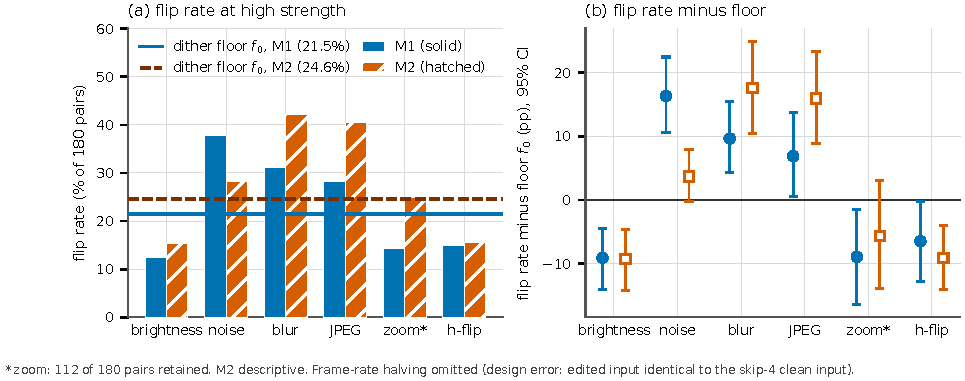
\includegraphics[width=\linewidth]{figures/f1_invariance.pdf}\caption{Flip rate per invariance edit at high strength, with the dither floor as a reference line. The frame-rate edit is a design error and is not interpreted.}\label{fig:f1}\end{figure}}{\par\noindent\textbf{[TODO figure F1: figures/f1\_invariance.pdf missing]}\par}
\IfFileExists{figures/f3_dose.pdf}{\begin{figure}[t]\centering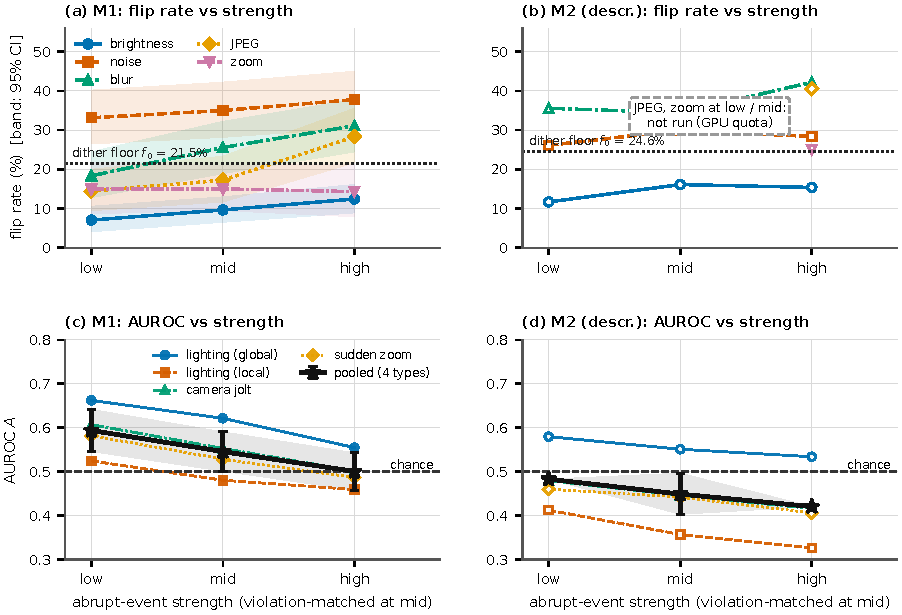
\includegraphics[width=\linewidth]{figures/f3_dose.pdf}\caption{Dose-response for M1: flip rate (invariance edits) and specificity AUROC (abrupt edits) against edit strength. Descriptive.}\label{fig:f3}\end{figure}}{\par\noindent\textbf{[TODO figure F3: figures/f3\_dose.pdf missing]}\par}

\else
\maketitle
\begin{abstract}
Violation-of-expectation (VoE) accuracy is often read as evidence that latent video world models represent intuitive physics. We ask what the underlying surprise signal of the public V-JEPA ViT-L checkpoint responds to, using three tests on frozen models: invariance to harmless edits, specificity against abrupt but possible events, and positive controls. On IntPhys dev, clean accuracy is 80.8\% in fp16 (81.7\% in fp32), well below the published 98\% for the larger ViT-H model, for a reason we could not identify; a copy-last-frame pixel baseline reaches 76.1\%. In fp16 inference, verdicts flip in 15.6\% (strict ties) to 21.5\% (tie-half) of pairs under an imperceptible one-grey-level dither. For near-threshold abrupt edits nominally matched in pixel magnitude, the surprise signal separates violations from edits with AUROC 0.546 (95\% CI 0.501 to 0.591), below our pre-registered detection precondition, so we could not determine whether it tracks physical impossibility or unpredictability. Our positive controls were not met. On IntPhys~2 Main, descriptively, the checkpoint is at chance (47.6\%). Results concern one public checkpoint, not latent world models in general.

\end{abstract}
\begin{IEEEkeywords}
intuitive physics, world models, V-JEPA, violation of expectation, video understanding
\end{IEEEkeywords}
\section{Introduction}
\label{sec:intro}
\begin{figure*}[t]
\centering
\IfFig{figures/f0_schematic.pdf}{Fig.~0 placeholder: a matched possible/impossible pair is scored by a predictor, giving a surprise curve; the three tests are invariance, specificity and positive controls.}
\caption{The violation-of-expectation protocol and the three tests we run. A model watches a possible and an impossible clip that look almost identical, and its prediction error (surprise) is compared. We ask whether that comparison survives harmless edits (invariance), whether it separates physics violations from abrupt but possible events (specificity), and whether it rises when we create a violation ourselves (positive controls).}
\label{fig:f0}
\end{figure*}

The violation-of-expectation (VoE) paradigm shows a model two videos that differ in one respect. In a typical IntPhys scene a ball rolls behind a screen; in the possible video it comes out the other side, and in the impossible one it vanishes. The videos are otherwise matched pixel for pixel \cite{riochet2022}. A model passes a pair if it is more surprised by the impossible video. The paradigm comes from developmental psychology and has been used to evaluate learned models of physics \cite{piloto2022,weihs2022}.

For video models that predict in a learned representation space, surprise has a concrete definition: the model sees the first frames of a clip, predicts the representation of what comes next, and the surprise at each moment is the distance between that prediction and the representation of what actually happens. Garrido et al.\ applied this to V-JEPA \cite{bardes2024} and reported a pairwise accuracy of 98\% on the IntPhys dev set for their flagship ViT-H model, with the context length tuned per property, with pixel-prediction and multimodal language-model baselines near chance, and above-chance results on two further benchmarks (GRASP and InfLevel-lab), without physics-specific training \cite{garrido2025}. This has been taken as evidence that predicting in latent space is enough to pick up some physical structure.

The accuracy number leaves a question open. A prediction error is large whenever the future is hard to predict. A ball that passes through a wall is impossible; a camera that jolts sideways is perfectly possible and still hard to anticipate. If the surprise signal responds to both, pairwise VoE accuracy on a benchmark whose impossible clips are also unpredictable could be high for reasons unrelated to physics. If it responds mainly to impossibility, the accuracy figure means what it appears to mean. Either answer is informative, and accuracy cannot distinguish them.

We train nothing. We test the surprise signal of frozen models directly, using deterministic edits to the IntPhys videos. The analysis plan and decision rules were pre-registered before any edited-condition output existed, with edit strengths calibrated on a separate split.

\begin{enumerate}
\item \textbf{Invariance.} Does the pairwise verdict survive edits that change appearance but not physics (blur, noise, compression, brightness, zoom, flips, frame dropping), applied identically to both clips of a pair?
\item \textbf{Specificity.} Does surprise separate real violations from physically possible abrupt events (a lighting step, a camera jolt, a sudden zoom) whose pixel change is scaled to match that of the violations, at near-threshold magnitude? Frame-difference baselines serve as a reference.
\item \textbf{Positive controls.} Does surprise rise when we create a violation ourselves, by flipping a clip vertically or reversing it in time? This checks that the pipeline can detect what it should.
\end{enumerate}

We run these tests on the public V-JEPA ViT-L checkpoint, which is the confirmatory model, and descriptively on V-JEPA~2 \cite{assran2025}, together with a randomly initialised network and trivial pixel baselines. Section~\ref{sec:method} describes the protocol. Our findings are limits on what the instrument can show. The public checkpoint does not reach the published ViT-H accuracy, its verdicts are not stable under an imperceptible perturbation, our positive controls were not met, and the pre-registered specificity test could not reach the detection level it requires, so it supports no claim in either direction. Sections~\ref{sec:results} and~\ref{sec:discussion} report all of this, including what the pre-registration did not anticipate.

\section{Related Work}
\label{sec:related}
\textbf{VoE benchmarks.} IntPhys pairs possible and impossible videos rendered in Unreal Engine, matched pixel for pixel, covering object permanence, shape constancy and continuity \cite{riochet2022}. InfLevel provides VoE experiments for continuity, solidity and gravity, on which the video architectures it tested were at or near chance \cite{weihs2022}. IntPhys~2 uses more complex scenes; V-JEPA and V-JEPA~2 are near chance on it (the best predictive model, V-JEPA~2, reaches 57.5\%), and a qualitative debug scene shows no extra surprise at the point where an occluded ball should reappear \cite{bordes2025}. Physion and Physion++ take another route: models predict object contact (and, in Physion++, infer latent properties such as mass and friction) and are compared with humans \cite{bear2021,tung2023}. We evaluate on IntPhys because its matched pairs make the pairwise verdict well defined.

\textbf{Latent prediction and intuitive physics.} V-JEPA learns video representations by predicting masked regions in representation space, with no pixel reconstruction \cite{bardes2024}; V-JEPA~2 scales the recipe to more video and adds a robot-planning stage \cite{assran2025}. Garrido et al.\ used V-JEPA's prediction error as a surprise signal and reported 98\% pairwise accuracy on IntPhys dev for their ViT-H model (context length tuned per property), with pixel-prediction and multimodal language-model baselines near chance \cite{garrido2025}. VideoMAE~V2, a masked autoencoder that reconstructs pixels, was planned as a pixel-reconstruction contrast model \cite{wang2023}; we did not run it. Joseph et al.\ probe video encoders layer by layer for physical information and find it concentrated at intermediate layers \cite{joseph2026}. These works report that the signal scores well on one benchmark. We ask what it responds to, for a public checkpoint.

\textbf{Doubts about what accuracy shows.} Su et al.\ report near-chance IntPhys~2 accuracy (0.50--0.54) for V-JEPA models trained on three different video sources, and note qualitatively that frame-wise surprise was often similar for possible and impossible videos \cite{su2025}. Li et al.\ find that on Physion, frozen V-JEPA~2 features with probes reach accuracy close to humans, while its disagreement with humans on individual items is far higher than between humans \cite{li2026}. That is a contact-prediction task, not a VoE one. Both point to the same gap: accuracy alone does not say what the model uses. We add one control for the VoE setting, abrupt edits to possible clips whose pixel magnitude is matched to the real violations.

\textbf{Counterfactual and likelihood-based evaluation of video models.} CRONOS probes whether video generators stay physically consistent under controlled visual interventions such as viewpoint, scene and appearance, and measures generation quality, not model surprise \cite{begiristain2026}. Physics-IQ evaluates the physical understanding of generative video models \cite{motamed2025}. LikePhys compares the denoising loss of matched valid and invalid videos for diffusion models \cite{likephys2025}. YoCausal treats denoising loss as surprise and uses time reversal of real videos as a counterfactual for diffusion models \cite{yocausal2026}. We use time reversal as one positive control; those results do not tell us whether it works for latent predictors, so we test it (Section~\ref{sec:method}). Our edits target the surprise of frozen predictive encoders.

\textbf{Impossible versus improbable.} Michaelov et al.\ found that language models do not reliably assign higher probability to possible-but-improbable sentences than to impossible ones \cite{michaelov2025}. Our specificity test asks the analogous question for video surprise.

\section{Method}
\label{sec:method}
All models are frozen; we run inference only. Every claim below concerns the public V-JEPA ViT-L checkpoint unless stated otherwise.

\subsection{Surprise}
We reuse the surprise computation of Garrido et al.\ \cite{garrido2025}. A predictor receives the representations of $M$ context frames and predicts the representations of the next $N$ frames. The surprise at time $t$ is the $L_1$ distance between the predicted and observed representation, $s_t=\lVert \hat z_t - z_t\rVert_1$ (averaged over tokens). A clip's score aggregates the window surprises: the mean over windows for clean accuracy and invariance (H1), and the maximum for specificity and positive controls (H2, H3; event-aligned for H2). The default score takes, per window, the minimum over context lengths $C\in\{2,4,6,8,10\}$ frames. Ablations A1 (aggregation) and A2 (one fixed context length $C\in\{2,6,10\}$ at a time) are in Supplement Table~S5. Models: V-JEPA ViT-L (M1) \cite{garrido2025,bardes2024}, V-JEPA~2 ViT-L (M2) \cite{assran2025}, VideoMAE~V2 (M3, planned \cite{wang2023} but not run), M1 with random weights (M0r), and two baselines: frame-difference surprise $\overline{|f_t-f_{t-1}|}$ (B1) and the pixel error of copying the last frame (B2).

\subsection{Data}
The main evaluation uses the IntPhys (2019) dev split \cite{riochet2022}, 180 pairs from 90 scene quadruplets (30 per block O1--O3). Edit strengths were calibrated on the 60-video IntPhys~2 Debug split \cite{bordes2025}, which is not used for evaluation. IntPhys~2 Main is used descriptively, for clean accuracy only; no edited runs were made on it (no event-time annotation). The IntPhys (2019) data are used as released for evaluation, and no videos are redistributed; the IntPhys~2 dataset card gives CC BY-NC 4.0. IntPhys~2 is used for evaluation only. In IntPhys dev, each impossible video is built by splicing frames of its possible partner videos (established by pixel hashing of the dev videos: 120 single and 60 double splices, none unspliced). This describes the dataset and is separate from the hypothesis, in the Discussion, that M1 relies on the splices.

\subsection{Edits}
Each edit is a deterministic function of frames, parameters and seed, applied before model preprocessing at three strengths (low, mid, high). Blur and low illumination at several graded severities are a common way to test vision models under degradation \cite{koushik2025,randieri2025}. Blur, JPEG and noise strengths are set on Debug frames to SSIM $0.95/0.85/0.70$ (JPEG high, $q=3$, reaches $0.689$ because quality is an integer); brightness gain to a mean CIELAB $L^*$ change of $5/10/20$; centre-crop scale is fixed at $0.9/0.8/0.7$. Horizontal flip, frame-rate halving and the dither floor have a single setting. \emph{Invariance edits} are applied with identical parameters and seed to both videos of a pair: brightness/colour shift, Gaussian blur, JPEG re-compression, additive Gaussian noise, centre crop and resize, horizontal flip, frame-rate halving (degenerate, see item~(f) of the deviations below). \emph{Abrupt edits} are applied to possible videos only, at an event time $t^*$: a persistent lighting step, camera jolt, or sudden zoom. The event time $t^*$ is the first frame at which the mean absolute pixel difference $D(t)$ between the impossible video and its prefix-sharing possible partner exceeds $\max(2/255,\ \text{the 99.9th percentile of } D \text{ over the first 10 frames of all pairs})$. If $D$ never exceeds this floor, the rule falls back to a seeded draw from the middle half of the clip. \emph{Positive controls}: vertical flip and time reversal of possible clips.

\emph{Magnitude matching.} For each pair, the violation's pixel change is $|\Delta|_{\mathrm{viol}}=\overline{|v_{\mathrm{imp}}-v_{\mathrm{pos}}|}$ over frames after the event, and the edit strength is solved so that the edit's mean pixel change over the same window equals the pair's violation magnitude (closed form for lighting, bisection for jolt and zoom); mid strength is $1\times$ this value, low $0.5\times$, high $2\times$. The pre-registered target is a median achieved-to-target ratio in $[0.95,1.05]$ with at least 90\% of pairs in $[0.9,1.1]$. Matching uses dev pixels only, never model output.

\subsection{Metrics and statistics}
\emph{Pairwise accuracy} is the fraction of pairs with $S(\text{impossible})>S(\text{possible})$; \emph{flip rate} is the fraction whose verdict differs from the clean one. We use McNemar tests against clean with Holm correction across edits. \emph{Specificity AUROC} is $P(\Delta_{\mathrm{viol}}>\Delta_{\mathrm{abrupt}})$ with $\Delta_{\mathrm{viol}}=S(\text{imp})-S(\text{pos})$ and $\Delta_{\mathrm{abrupt}}=S(\text{pos+edit})-S(\text{pos})$, with a 10{,}000-resample bootstrap 95\% CI; the $D_1$ and $D_2$ contrasts use a one-sided paired bootstrap $p$-value (floor $2\times10^{-4}$) and a paired CI. \emph{Detection rate} for positive controls is the fraction of videos with $S(\text{edited})>S(\text{original})$ with a binomial CI. Edit randomness uses 3 seeds (sign, colour direction, noise realisation, jolt direction); deterministic edits run once. The bootstrap resamples scene quadruplets, stratified by block. Ties are scored 0.5 (``tie-half'') when two scores differ by at most $2\times10^{-4}$ times the median clean score of that type; a strict convention ($<$, as in the released code) and an exact-tie convention ($\tau=0$) are sensitivity analyses, and we report the tie-half and strict figures for the dither floor.

\subsection{Pre-registration}
Edit parameters, seeds, metrics, analysis plan and thresholds were frozen on 7 October 2026 at commit \texttt{ee63aee} (tag \texttt{prereg-frozen}), before any edited-condition output existed. Strengths were calibrated on IntPhys~2 Debug only. Decision rules, as frozen:
\begin{itemize}
\item \emph{Invariance (H1).} An edit is ``violated'' if accuracy drops by at least 5 points with a Holm-adjusted scene-cluster bootstrap $p<0.05$, or if its flip rate is at least 10\% and at least 5 points above the dither floor with Holm-adjusted $p<0.05$; it is ``invariant'' if the accuracy lower bound exceeds $-5$ points and the upper bound of flip minus floor is below 5 points. The Holm family has 14 tests (7 edits $\times$ accuracy and flip). If the dither floor is at least 10\%, H1 for that model is descriptive.
\item \emph{Specificity (H2).} Let $A$ be the specificity AUROC of M1, and $A_0$ the clean pairwise accuracy of M1 under the same event-aligned max aggregation (detection precondition). Define $D_1=A_{\mathrm{M1}}-A_{\mathrm{B1}}$ and $D_2=A_{\mathrm{M1}}-A_{\mathrm{B2}}$. ``Specific'' requires $A\ge0.80$, both $D_1$ and $D_2$ significant under Holm correction over these two tests, and per-type AUROC of at least 0.65; $0.65<A<0.80$ is partial; $A\le0.65$ is not specific. If $A_0<0.85$ and the table yields not specific or partial, the outcome is ``detection-limited'': specificity cannot be assessed and no claim is made in either direction. This Holm-2 rule replaced an earlier intersection-union rule before the freeze.
\item \emph{Positive controls (H3, gate G2).} Vertical flip must raise M1's surprise in at least 80\% of possible videos, with the lower confidence bound against horizontal flip above 0.5.
\end{itemize}
A model is H1-eligible only if its clean accuracy is at least 80.0\%. Analyses outside this plan are labelled exploratory.

\subsection{Deviations, amendments and known design weaknesses}
\label{sec:deviations}
Each item departs from the plan or limits what a result can show, and is carried into Section~\ref{sec:discussion}. Full descriptions are in Supplement Section~S-I.
(a)~\emph{Checkpoint gap (G1$'$).} The original gate (at least 90\% on IntPhys dev) was not met: the public ViT-L checkpoint reaches 81.7\% (ViT-H 88.3\%, tie-half under the pre-registered threshold). The checkpoints behind the published results are not released and the gap is unexplained; we do not claim a reproduction of the published 98\%, which is for ViT-H with per-property context length. The replacement gate G1$'$ checks the pipeline only, and all three of its checks passed.
(b)~\emph{Positive controls (G2 not met).} Vertical flip raised M1's surprise in 21.1\% of possible videos against the 80\% gate, and pairwise accuracy on flipped pairs is not lower than clean. Three readings remain open (the edits are weak violations for this model; the pipeline is insensitive; the signal acts as a splice-discontinuity detector), so M1's sensitivity to physical impossibility is not established. By human decision (Q10-A, logged 2026-10-08) the study continued with G2 not met, so every H1 and H2 statement carries this caveat. The random-weight network M0r responds in 87.8\% of videos where about 50\% was expected, so M1 minus M0r is not a measure of learned sensitivity.
(c)~\emph{Magnitude matching in H2.} The frozen event rule fell back to a seeded random onset in 178 of 180 pairs. This is a failure of the rule, not a finding that no event exists. The median matched magnitude is 0.33 of 255 grey levels, so the edits are near-threshold; for global lighting, 84 of 180 entries are no-ops, so $A$ is reported with and without that type. Both pixel baselines fall below 0.5 for a reason we did not verify.
(d)~\emph{M2 wrapper.} The first V-JEPA~2 run used mask token index~1, but only token~0 is trained. After the freeze we changed it to~0 (human-approved, logged before any edited M2 output was opened) and reran the clean split: 46.9\% before, 60.8\% after. Both are reported; M2 is not H1-eligible.
(e)~\emph{Invariance is descriptive.} The dither floor of 21.5\% (15.6\% strict) exceeds 10\%, so every edit is read through its accuracy change and its flip rate relative to the floor. The floor was measured in fp16 only. For JPEG the verdict depends on the tie convention, and for zoom a retention rule leaves 112 of 180 pairs.
(f)~\emph{Frame-rate edit (design error).} The pre-registered edit reproduces the skip-4 clean reference bit-identically, so its zero change cannot be read as invariance; it is excluded from all counts.
(g)~\emph{Other.}
\begin{itemize}
\item Holm families. H1 primary: 14 tests. H1 dose-response: 30 tests for M1 (the pre-registration names 21, but only 15 graded cells exist) and 22 for M2 (11 cells, two tests each). H2 dose-response: 24 tests at cell level and 6 for the pooled contrasts. The M2 dose cells are seed 1 only.
\item Precision. H1 eligibility was judged on the fp32 clean run and contrasts use fp16; the G1$'$ ladder compares ViT-L in fp32 with ViT-H in fp16.
\item Logistics. Kernel bundles were rebuilt at later commits with the commit allowlist extended (human decision Q10-C: ``proceeds''); the per-pair matching file was generated after the freeze from dev pixels only; the Colab fallback was not used. H2 was run as frozen, with its weaknesses disclosed, by human decision (Q11).
\end{itemize}
Exploratory analyses are labelled wherever they appear; the IntPhys~2 Main clean run is descriptive, as pre-registered.

\section{Results}
\label{sec:results}
Unless stated otherwise, results are for the public V-JEPA ViT-L checkpoint (M1) on the 180 IntPhys dev pairs. Percentages use the tie-half convention (Section~\ref{sec:method}); strict-convention values are given where they differ. Confidence intervals are 95\% scene-cluster bootstrap intervals. Under the pre-registered rules, H1 (invariance) is descriptive for M1, H2 (specificity) is detection-limited, and gate G2 was not met; read every statement below with that in mind.

\subsection{Clean accuracy and baselines}
\label{sec:res-clean}
Clean pairwise accuracy of M1 is 81.7\% in fp32 (80.6\% strict) and 80.8\% in fp16 (81.1\% strict); the fp16 run is the reference for all contrasts. The published 98\% (ViT-H) is not reproduced (Section~\ref{sec:deviations}). The public ViT-H checkpoint, the like-for-like comparison, reaches 88.3\% (87.8\% strict). The copy-last-frame baseline B2 reaches 76.1\%, and the windowed frame-difference baseline B1 reaches 58.1\% (57.2\% strict). The paired difference between M1 (fp16) and B2 is +4.7 pp with a confidence interval of $-$1.1 to 10.6 pp, which includes zero; against the fp32 run it is +5.6 pp (0.0 to 11.1), with the lower bound at zero. Clean accuracy does not separate M1 from a copy-last-frame pixel baseline. V-JEPA~2 (M2) reaches 60.8\% after the mask-token correction (60.6\% strict; 46.9\% before it) and is not H1-eligible. VideoMAE~V2 (M3) was not run. Table~\ref{tab:t1} lists all rows.

\IfFileExists{tables/t1_reproduction.tex}{\begin{table}[t]
\caption{Reproduction on IntPhys dev (180 pairs, 3 blocks): pairwise accuracy in \% of the impossible video having the higher surprise (mean aggregation; tie-half = primary, strict = ties counted wrong). Published: Garrido et al.\ headline $\approx$98\%, obtained with checkpoints that are not released; the gap to our public checkpoints is unexplained and we make no reproduction claim. M1 minus B2 (paired): +4.7 pp [$-$1.1, 10.6].}
\label{tab:t1}
\centering\scriptsize
\setlength{\tabcolsep}{2.5pt}
\begin{tabular}{@{}lrrr@{}}
\toprule
Model & Tie-half & Strict & Published \\
\midrule
M1 V-JEPA ViT-L, fp32 & 81.7 & 80.6 & $\approx$98$^{\rm a}$ \\
M1 V-JEPA ViT-L, fp16 & 80.8 & 81.1 & -- \\
M1H V-JEPA ViT-H (diagn.)$^{\rm b}$ & 88.3 & 87.8 & -- \\
M2 V-JEPA 2 ViT-L & 60.8 & 60.6 & -- \\
M3 VideoMAE V2 & \multicolumn{2}{c}{\textit{not run}} & -- \\
M0r random init (3) & 50.0 & 50.2 & expected $\approx$50 \\
B1 frame difference & 58.1 & 57.2 & expected $\approx$50 \\
B2 copy-last-frame & 76.1 & 76.1 & -- \\
\midrule
\multicolumn{4}{@{}l}{\textit{Superseded, disclosure only (not the M2 number)}} \\
M2 old run (mask idx 1)$^{\rm c}$ & 46.9 & 46.7 & -- \\
\bottomrule
\end{tabular}
\vspace{2pt}

\raggedright\scriptsize $^{\rm a}$Literature value, not our run. $^{\rm b}$Prereg-tau tie-half 88.3; the 88.1 in the pre-registration text is the superseded fixed-$\tau$ figure (strict 87.8). $^{\rm c}$Wrapper deviation (query mask index 1), excluded from every M2 contrast.
\end{table}
}{\par\noindent\textbf{[TODO table T1: tables/t1\_reproduction.tex missing]}\par}

\subsection{Invariance (H1): descriptive}
\label{sec:res-h1}
The verdict flip rate under an imperceptible $\pm1$ grey-level dither is 21.5\% (15.6\% strict), above the 10\% limit, so invariance for M1 is descriptive and we report accuracy changes and flip rates relative to this floor (Table~\ref{tab:t2}; Fig.~S1 in the supplement). We do not assign the driver's verdict labels. At high strength, additive noise lowers accuracy by $-$20.6 pp ($-$25.7 to $-$15.3) with a flip rate of 37.8\%, +16.3 pp above the floor (10.6 to 22.4). Blur lowers accuracy by $-$14.4 pp ($-$19.4 to $-$9.4; flip 31.1\%, +9.6 pp above the floor), and JPEG by $-$10.8 pp ($-$16.4 to $-$5.3; flip 28.3\%, +6.9 pp above the floor). For JPEG the Holm-adjusted accuracy test depends on the convention: under tie-half the cluster and sign tests give $p$ $<$0.0001 and 0.018, under the strict convention 0.0088 and 0.1151. Brightness changes accuracy by $-$2.4 pp ($-$5.1 to 0.3; flip 12.4\%), horizontal flip by +2.2 pp ($-$2.2 to 6.7; flip 15.0\%) and centre crop by $-$0.5 pp ($-$5.7 to 4.9; flip 14.3\%, on 112 of 180 pairs after the retention exclusion). For these three, the flip rate is at or below the dither floor, so the edit adds no flips beyond the floor. The frame-rate edit is bit-identical to its reference by a design error and tests nothing; it is excluded here.

\emph{Dose-response (A3, descriptive).} Accuracy loss grows with strength for blur ($-$4.7, $-$11.9, $-$14.4 pp at low, mid, high); for JPEG the change is +5.8, +0.8 and $-$10.8 pp, so a loss appears only at the highest setting. Noise is already at $-$17.7 pp at the lowest strength (flip 33.2\%), and brightness stays within a few points of zero at all strengths, with low- and mid-strength flip rates (7.0\% and 9.6\%) below the floor. The family is Holm over 30 tests (Section~\ref{sec:deviations}; Table~S4 and Fig.~S2 in the supplement).

\IfFileExists{tables/t2_invariance.tex}{\begin{table*}[t]
\caption{Invariance (H1), high strength. $\Delta$Acc = accuracy under the same edit applied to both videos of a pair minus clean accuracy, in percentage points (scene-cluster 95\% CI); flip = share of pairs whose verdict changes; flip$-f_0$ = flip rate minus the dither floor $f_0$ (a perturbation that should not matter at all): M1 $f_0$ = 21.5\% (strict 15.6\%), M2 $f_0$ = 24.6\%. A flip rate near $f_0$ is what an invisible perturbation produces. Holm-14 adjusted $p$ for $\Delta$Acc / flip. M1 is the confirmatory row; M2 is \textbf{descriptive only} (clean accuracy below the 80\% eligibility rule).}
\label{tab:t2}
\centering\scriptsize
\setlength{\tabcolsep}{1.9pt}
\begin{tabular}{@{}lrrrrrrrr@{}}
\toprule
 & \multicolumn{4}{c}{M1 V-JEPA ViT-L} & \multicolumn{4}{c}{M2 V-JEPA 2 (descriptive)} \\
\cmidrule(lr){2-5}\cmidrule(lr){6-9}
Edit ($n$ pairs) & $\Delta$Acc [CI] & Flip & Flip$-f_0$ [CI] & $p$ ($\Delta$/flip) & $\Delta$Acc [CI] & Flip & Flip$-f_0$ [CI] & $p$ ($\Delta$/flip) \\
\midrule
Brightness (180) & $-$2.4 [$-$5.1, 0.3] & 12.4 & $-$9.1 [$-$14.1, $-$4.4] & 0.63 / 1.00 & $-$0.4 [$-$3.1, 2.5] & 15.4 & $-$9.3 [$-$14.3, $-$4.6] & 1.00 / 1.00 \\
Noise (180) & $-$20.6 [$-$25.7, $-$15.3] & 37.8 & +16.3 [10.6, 22.4] & $<$0.001 / $<$0.001 & $-$6.4 [$-$11.5, $-$1.3] & 28.3 & +3.7 [$-$0.2, 8.0] & 0.13 / 0.30 \\
Blur (180) & $-$14.4 [$-$19.4, $-$9.4] & 31.1 & +9.6 [4.3, 15.4] & $<$0.001 / 0.001 & +12.8 [6.4, 19.2] & 42.2 & +17.6 [10.4, 24.8] & $<$0.001 / $<$0.001 \\
JPEG (180) & $-$10.8 [$-$16.4, $-$5.3] & 28.3 & +6.9 [0.6, 13.7] & $<$0.001 / 0.15 & $-$1.7 [$-$7.8, 4.4] & 40.6 & +15.9 [8.9, 23.3] & 1.00 / $<$0.001 \\
Zoom (crop)$^{\rm a}$ (112) & $-$0.5 [$-$5.7, 4.9] & 14.3 & $-$8.9 [$-$16.4, $-$1.6] & 1.00 / 1.00 & +7.1 [1.7, 12.8] & 25.0 & $-$5.7 [$-$13.9, 3.1] & 0.13 / 1.00 \\
Horiz.\ flip (180) & +2.2 [$-$2.2, 6.7] & 15.0 & $-$6.5 [$-$12.8, $-$0.2] & 1.00 / 1.00 & +3.3 [$-$0.3, 6.9] & 15.6 & $-$9.1 [$-$14.1, $-$4.1] & 0.58 / 1.00 \\
\bottomrule
\end{tabular}

\vspace{2pt}
\raggedright\scriptsize Flip and flip$-f_0$ in \%, $\Delta$Acc in pp. $^{\rm a}$Pairs where the crop keeps the scene support (112 of 180); the other 68 are excluded for both models. Frame-rate halving is not tabulated: its edited input is bit-identical to the skip-4 clean reference, so the edit is degenerate by design (a design error in the edit list, reported here for completeness).
\end{table*}
}{\par\noindent\textbf{[TODO table T2: tables/t2\_invariance.tex missing]}\par}

\subsection{Positive controls (H3, gate G2): not met}
\label{sec:res-h3}
Vertical flip raises M1's surprise in 21.1\% of possible videos (14.7 to 28.1), far below the 80\% gate; against the horizontal-flip reference the rate is 25.8\% (18.6 to 33.3). Horizontal flip itself gives 38.6\%. Time reversal, reported but not gating, gives 60.8\% (51.7 to 69.4). Pairwise accuracy on vertically flipped pairs is 83.9\%, not lower than the clean 80.8\%. The random-weight network M0r raises its surprise under vertical flip in 87.8\% of videos (82.2 to 93.1), where the pre-registration expected about 50\%; the M1 minus M0r difference in detection is $-$66.7 pp ($-$76.1 to $-$56.7), and we do not interpret it as a measure of learned sensitivity. G2 was not met. We cannot show that the pipeline responds to physical violations other than the dataset's own frame splices (Table~S2 in the supplement).

\subsection{Specificity (H2): detection-limited}
\label{sec:res-h2}
The test uses the 180 possible videos. The event rule fell back to a random onset in 178 of 180 pairs, and the median matched magnitude is 0.33 grey levels of 255, so the edits are near-threshold. For global lighting, 84 of 180 entries are no-ops after rounding. The specificity AUROC of M1 is $A=$0.546 (0.501 to 0.591), and 0.520 (0.475 to 0.565) without global lighting. Per type it is 0.622 (global lighting), 0.480 (local lighting), 0.553 (camera jolt) and 0.528 (zoom); the global-lighting value largely measures clean detection and is not evidence of partial specificity. The detection precondition is not met: clean accuracy under the same aggregation is $A_0=$0.722 (0.664 to 0.781) against the required 0.85. By the pre-registered rule the outcome is \emph{detection-limited}: specificity cannot be assessed here and we make no claim in either direction. The outcome is the same under the strict and exact-tie conventions and with global lighting excluded. Ablations over aggregation and fixed context length are in Supplement Table~S5, and results per block in Table~S6.

Both pixel baselines fall below chance, with $A_{B1}=$0.335 and $A_{B2}=$0.379. The contrasts $D_1=$+0.211 (0.159 to 0.263) and $D_2=$+0.166 (0.116 to 0.219) are Holm-significant ($p=$0.0002, the bootstrap floor), but this reflects the baselines' distance below 0.5 under this matching, not evidence about M1; we do not read them as M1 outperforming a baseline. As a function of edit strength, $A$ is 0.594 (0.546 to 0.642) at half the matched magnitude, 0.546 at the matched magnitude and 0.501 (0.458 to 0.543) at twice, and it falls with strength in all four types (descriptive; Holm over 24 tests, all at the bootstrap floor). Figure~\ref{fig:f2} shows the distributions, and Table~S3 in the supplement lists the per-type values, the M2 rows and the analysis without global lighting.

\IfFileExists{figures/f2_specificity.pdf}{\begin{figure*}[t]\centering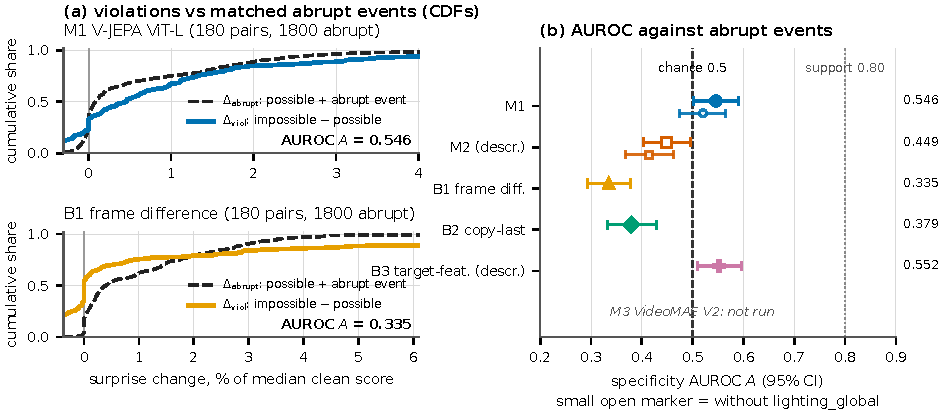
\includegraphics[width=\textwidth]{figures/f2_specificity.pdf}\caption{Specificity (H2) for M1 and the pixel baselines: distributions of $\Delta_{\mathrm{viol}}$ and $\Delta_{\mathrm{abrupt}}$, and AUROC with 95\% intervals. Baselines below 0.5 reflect the matching, not model skill.}\label{fig:f2}\end{figure*}}{\par\noindent\textbf{[TODO figure F2: figures/f2\_specificity.pdf missing]}\par}

\subsection{V-JEPA~2 (M2): descriptive}
\label{sec:res-m2}
M2 is H1-ineligible (clean 60.8\%), so all M2 results are descriptive. Its dither floor is 24.6\%. Its specificity AUROC is 0.449 (0.403 to 0.496), 0.415 without global lighting, with $A_0=$0.600 (0.542 to 0.658); the rule again gives the detection-limited outcome, and the upper interval bound lies below 0.5. Both pixel baselines are again below 0.5 (0.324 and 0.376).

\emph{M2 positive controls.} Vertical flip raises M2's surprise in 71.9\% of videos (64.4 to 78.9), reversal in 46.4\% (38.6 to 54.2); G2 is not met for M2 either, and M2 minus M0r is $-$15.8 pp ($-$25.0 to $-$6.7). Pairwise accuracy on its vertically flipped pairs is 64.4\%. The M2 dose-response (seed 1 only, descriptive) is in Supplement Section~S-II. Because M2 is ineligible and does not meet G2, no statement here extends to latent world models in general.

\subsection{IntPhys 2 Main: descriptive}
\label{sec:res-ip2}
On the 506 IntPhys~2 Main pairs, M1's clean accuracy is 47.6\% (43.7 to 51.7; 47.8\% strict), at chance. The pixel baselines are also at chance (B1 51.2\%, B2 51.9\%, B3 46.6\%). By category M1 scores 46.7\% (continuity), 42.1\% (immutability), 49.6\% (permanence) and 51.4\% (solidity). Removing the four pairs whose names overlap the Debug split changes nothing material (47.6\%). The verdict is at chance here, which limits what the signal can show; we draw no further conclusion from it. We did not run the specificity test on this split (no event-time annotation).

\subsection{Exploratory analyses}
\label{sec:res-expl}
These were run after the confirmatory results were seen and are exploratory (details and Table~S1 in Supplement Section~S-II). An onset-aligned specificity variant, using the splice time derived from prefix-sharing frames of the dev pixels, gives an AUROC for M1 of 0.392 (0.354 to 0.428), lower than with random windows (0.546), with the detection precondition unchanged ($A_0=$0.722), so the rule's outcome does not change; both baselines stay below 0.5. An AUROC below 0.5 means that the matched possible edits raise surprise more than the violations do. M2's AUROC (0.449, upper bound 0.496) is also below 0.5. Under the frozen table this pattern carries the sub-label ``Reversed''; because the detection precondition is unmet, the confirmatory M1 outcome stays detection-limited and we draw no conclusion from it. A hold-based frame-rate edit that differs from the skip-4 reference changes accuracy by +1.9 pp ($-$3.3 to 7.5) with a flip rate of 20.0\%, within the 21.5\% floor. The fp32 flip rate was not measured. A paired check on the stored arrays shows that M0r's surprise shifts systematically in one direction under vertical flip, opposite to M1's shift, and not through ties or noise; the cause is not established.

\section{Discussion and Limitations}
\label{sec:discussion}
\textbf{What the data show.} For the public V-JEPA ViT-L checkpoint we can state four things. First, its clean pairwise accuracy on IntPhys dev (81.7\%) is well below the published ViT-H figure (98\%), and it is not separable from a copy-last-frame pixel baseline (76.1\%; paired difference +4.7 pp, interval $-$1.1 to 10.6). Second, the verdict is unstable under a dither no viewer could see (21.5\% of pairs flip, 15.6\% strict), so any statement that a verdict is robust or fragile to an edit must be made against that floor. Third, our positive controls were not met: vertical flip raised surprise in 21.1\% of videos against a gate of 80\% (time reversal, not gating, 60.8\%), while a randomly initialised network did respond to vertical flip (87.8\%). Fourth, the pre-registered specificity rule returns ``detection-limited'': $A=$0.546 (0.501 to 0.591), and 0.520 (0.475 to 0.565) without global lighting, with a clean detection precondition of 0.722 against the required 0.85. Under the rule, specificity cannot be assessed here, and we make no claim in either direction: we do not claim that the signal tracks unpredictability rather than impossibility, nor the reverse.

\textbf{How these fit together.} The results are consistent with a reading in which the pairwise verdict on IntPhys dev relies largely on the discontinuities that the dataset's frame splices create. That the dataset is built from splices is a measured property of the dev videos (Section~\ref{sec:method}); that M1 relies on them is a hypothesis. A clip flipped vertically or reversed in time is internally consistent and has no such discontinuity. M1's surprise does not rise under vertical flip: in an exploratory paired check on the stored arrays its surprise decreases in 79.4\% of possible videos, while the random-weight network's increases in 87.8\%, and the cause is not established. Its accuracy on flipped pairs (83.9\%) does not fall. Time reversal, which also contains no splice, raises M1's surprise in 60.8\% of videos (lower confidence bound 51.7\%); this modest rise is not what a splice-only reading predicts, so the hypothesis is at best partial. A copy-last-frame baseline, which also responds to discontinuities, reaches a similar accuracy; M1 and B2 are not distinguishable at 180 pairs, which is not evidence that they are equivalent. We label the splice reading a hypothesis: our data do not rule out other explanations, and we did not test it directly. The random-weight network's response indicates that vertical flip changes something an untrained network also responds to, so the flip control is weaker than intended whatever M1 does.

\textbf{Exploratory splice analysis (post hoc, uncorrected, $n=180$).} Every one of the 180 impossible dev videos is a splice of its possible partners (120 single, 60 double). M1's accuracy is 91.2\% on the 137 pairs that the copy-last-frame baseline B2 gets right and 47.7\% on the 43 it gets wrong, and the per-pair margins of M1 and B2 correlate (Spearman 0.54, 0.42 to 0.65). M1 scores 75.0\% on single and 92.5\% on double splices, while B2 scores 75.0\% and 78.3\%. The window of peak surprise contains a switch frame in 73.9\% of impossible videos against 46.9\% expected by chance, and accuracy shows no monotone pattern across terciles of the splice position. Vertical flip changes few verdicts net (11 lost, 13 gained; McNemar $p=0.84$), whereas time reversal loses 23 pairs and gains 9 ($p=0.02$). These are associations. They do not separate ``M1 detects the cut'' from ``M1 and B2 both respond to post-splice scene differences'', and we do not take them as showing or establishing the splice reading. A causal test needs impossible videos that are not splices, which this dataset does not contain. On IntPhys~2 Main, M1 is at chance (47.6\%, 43.7 to 51.7); this agrees in direction with earlier reports of near-chance V-JEPA accuracy on that benchmark \cite{bordes2025,su2025}, and we draw no causal link.

\textbf{What this implies for how VoE results are reported.} A single pairwise accuracy cannot tell a model that tracks impossibility from one that tracks something correlated with it. We suggest reporting, next to accuracy, (i) the noise floor of the verdict under an imperceptible perturbation, (ii) the accuracy of trivial pixel baselines on the same pairs, and (iii) a positive control, with a randomly initialised model alongside it. None of these needs training. Our matching of abrupt edits on mean pixel difference was not sufficient: both pixel baselines landed below chance, so equal mean change does not mean equal visibility to every detector. A matched-event test with annotated event times and edits above the visibility threshold is a natural next step.

\textbf{Scope.} These conclusions concern one public checkpoint, on synthetic scenes, with frozen inference. V-JEPA~2 was run descriptively and is not H1-eligible, so nothing here extends to latent world models in general.

\subsection{Limitations}
\label{sec:limitations}
These limit every conclusion; details are in Section~\ref{sec:deviations}. (i) One public checkpoint, whose accuracy (81.7\%) falls short of the published ViT-H figure for an unexplained reason. (ii) The positive controls were not met, so we cannot show a response to violations beyond the dataset's frame splices; in IntPhys dev a ``violation'' is a splice. (iii) The specificity edits are near-threshold (median 0.33 of 255 grey levels) and placed at random windows for 178 of 180 pairs, and global lighting is a no-op in 84 of 180 entries. (iv) The H2 tie threshold ($1.09\times10^{-4}$) is small against the fp16 margin noise (up to $5.5\times10^{-4}$ per pair), so many effects of this size lie near the numerical floor. (v) Both pixel baselines are below chance, so $D_1$ and $D_2$ are artefact-prone. (vi) Invariance is descriptive: the dither floor exceeds 10\% and was measured in fp16 only, the zoom edit rests on 112 of 180 pairs, and the frame-rate edit is degenerate by our design error. (vii) M2 is H1-ineligible and descriptive, and M3 was not run. (viii) Seed variation covers nuisance parameters only and is not uncertainty; the scene bootstrap carries it. (ix) Synthetic scenes, one dataset for the main claims, frozen models, four abrupt-event types.

\fi
\ifsupp\else
% AUTHOR TO WRITE: AI-use disclosure / Acknowledgements section goes here (left blank on purpose).

\noindent\textbf{Reproducibility.} The design was frozen at commit \texttt{ee63aee}; inference ran on Kaggle GPUs in fp16 with an fp32 check. Analysis code, the pre-registration and verification scripts are at \texttt{github.com/anand-r-m/vjepa-surprise-physics}; per-video surprise arrays are available on request. Videos are not redistributed.
\IfFileExists{refs.bib}{\bibliographystyle{IEEEtran}{\footnotesize\bibliography{refs}}}{\bibliographystyle{IEEEtran}\bibliography{refs_writer_stub}}
\fi
\end{document}
